%!TEX root = /Users/simo/Documents/PFC/Chapter1/chapter1.tex

\section{Diseño} % (fold)
\label{sec:diseno}
Como buen proyecto de desarrollo de una aplicación, se pretende seguir los pasos naturales comunes a todos los proyectos de este tipo. Primero se establecieron una serie de criterios en la etapa de especificación. Seguidamente hubo un proceso de comprensión de las tecnologías para ver las diferencias en el proceso de desarrollo de una aplicación web respecto a las aplicaciones más clásicas. Y finalmente solo queda realizar una etapa de diseño que, en mayor o menor medida, ayude a planear un desarrollo estructurado de esta aplicación.

Como en etapas anteriores, también es posible enfocar el diseño de esta aplicación como dos elementos bastante diferenciados, y que necesitarán de un proceso de desarrollo suficientemente independiente como para ser considerados por separado. Es cierto que deberán interactuar, y por eso se incluye un apartado que pretende entender de qué forma se llevará a cabo esta comunicación, y de qué manera afectará al enfoque que se le deba dar en cuanto al desarrollo.

\subsection{Pizarra}
Se ha explicado con anterioridad las características de Javascript, el cual, a pesar de sus limitaciones, es orientado a objetos, y es posible programar de forma bastante modular gracias a ello. Un boceto inicial de lo que podría ser el diagrama de clases del dominio se puede encontrar en la figura \ref{fig:jsdom1}.

\begin{figure}[h!]
\centering
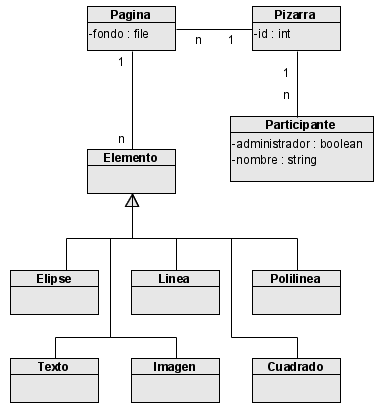
\includegraphics[width=10.5cm]{javascript-dominio1.png}
\caption{Boceto de clases del dominio}\label{fig:jsdom1}
\end{figure}

Cada Pizarra es única, tiene su identificador, y en la que participan una serie de usuarios. Dicha Pizarra tiene una serie de páginas, y un fondo opcional. Este fondo se generará si el creador de la pizarra ha subido un documento que sirva de fondo (recordando, un PDF, powerpoint, o simplemente una serie de imágenes). A partir de ahí, simplemente habrá una serie de elementos, que podrán ser de distinto tipo. Es difícil de definir en estos momentos qué atributos deben tener estos elementos, pues dependen en gran medida de las forma en que están implementados en SVG o VML.

Hay una parte importante de la especificación de las funciones de la pizarra que se ha considerado opcional, y por eso no aparece aquí. Por ejemplo, si se llegara a implementar un chat, y se guardara registro, harían falta clases extra. En cualquier caso, este diagrama da una buena idea de los elementos que se manejarán a lo largo del uso de la Pizarra.

Una vez sabido esto, el código que manejará estos elementos se distribuirá en una serie de módulos. Hay que recordar que la Pizarra está integrada en un sistema, que es la página web, que le proveerá con la información necesaria. Por ejemplo, Javascript de por si no es capaz de consultar una base de datos, pero si consultar otra página mediante Ajax, que le devuelva lo que necesita saber. Dicha página será generada por el Sistema, que en este caso funcionará bajo Ruby on Rails, que será el que consultará la base de datos y genere los datos con el formato adecuado para que Javascript lo pueda entender.

\begin{description}
	\item[Renderizado] Aquí se agruparán las funciones que dibujen los elementos. Debe tener las funciones necesarias para poder dibujar los elementos que se soporten (líneas, polilíneas, cuadrados, círculos, etc), así como editarlos, y que sea capaz de hacerlo independientemente del navegador que se esté usando.
	\item[Dibujo] Será el módulo que controle los eventos del ponente. Debe ser capaz de entender los movimientos de ratón y teclado de forma que indique al módulo de renderizado las figuras que debe crear de forma que se experimente una sensación de dibujo interactivo. Además, debe de comunicar al sistema cuándo se ha creado, editado, o eliminado algún elemento.
	\item[Comunicación] Éste módulo incluirá las funcionalidades de comunicación entre la interfaz, en javascript (recordando que javascript es incapaz de consultar bases de datos), y el sistema web. Será capaz de informar en ambas direcciones, tanto cuando el ponente ha modificado la pizarra para decírselo al sistema, como cuándo el sistema recive nuevos elementos, para comunicárselos a los espectadores.
	\item[Controlador de Usuarios] Debe de controlar los usuarios que el sistema le dice que entran a la Pizarra, y darles los privilegios adecuados. Debe de mostrarlos en la pizarra para informar a los demás.
\end{description}

Debido a las características peculiares de Javascript, se considera este enfoque como el más sencillo y eficiente para un programador con conocimientos escasos del lenguaje. El hecho de que javascript sea orientado a objetos, permite que se creen clases adecuadas para por ejemplo representar las clases del dominio, sin embargo, sigue siendo más sencillo implementar dichos controladores como una serie de funciones agrupadas en un archivo, más que hacer realmente una clase Renderizado, con subfunciones. En cualquier caso, se dará una gran importancia a intentar implementar de forma coherente con el paradigma de orientación a objetos, en la medida de lo posible acorde con las características de Javascript, y el nivel de conocimiento del lenguaje del programador. En esta fase del desarrollo es difícil definir hasta qué punto será posible.


\subsection{Sistema}

El sistema debe servir como intermediario entre todos los usuarios que participan en una pizarra, y ser capaz de realizar las funciones que Javascript, de por si solo, no es capaz. Antes de empezar a participar en alguna pizarra hay una serie de acciones que deben de ser controladas por el sistema. Dichas funcionalidades se pueden recoger en una serie de módulos, los cuales más adelante se intentarán formalizar en una estructura compatible con el paradigma Modelo-Vita-Controlador de Rails.

\begin{description}
	\item[Control de Usuarios y Grupos] Es necesario mantener un control de los usuarios y los grupos a los que se pertenece, y para ello es necesario una base de datos. Los usuarios tienen que poder registrarse y hacer las funciones típicas, como Login, edición de datos, creación de grupos, etc. Éste módulo debería ser capaz de controlar todo lo referente a usuarios y grupos según el comportamiento que se ha definido anteriormente.
	\item[Control de Pizarras] Las responsabilidades de este módulo serían las de mantener un control de las pizarras que existen, sus permisos, y su contenido. Cada pizarra tiene una serie de páginas, y cada página una serie de elementos, que deben de ser accesibles y modificables, así como poder crear o eliminar nuevos.
	\item[Comunicación con Javascript] Ésta es la funcionalidad más importante, y a falta de un nombre más apropiado, este módulo debe hacer precisamente esto, ser capaz de comunicarse con la interfaz, que se está ejecutando en el cliente, y no en el servidor. Debido a las características de Ajax y de Rails, se cree que no será posible separar formalmente estas funcionalidades, y que deberá ser incluida en los otros dos módulos. La sección siguiente ayudará a entender porqué.
\end{description}

\subsubsection{Entendiendo AJAX}
Antes de seguir se considera interesante entender como funciona Ajax, pues es la única técnica conocida que permite la interactividad que se espera de un programa como el que se está desarrollando, pero a su vez hace que se deban enfocar las cosas de una forma un poco distinta al paradigma típico de Cliente-Servidor.

Para empezar, hay que entender que la forma en que uno navega por la web, es consultando distintas páginas, una a una. La única forma de que un servidor es capaz de comunicarse con un usuario, es cuando este usuario le ha hecho alguna consulta. No existe forma alguna de que un servidor abra una conexión hacia un usuario por voluntad propia. Típicamente, cuando se navega, se consulta una página, que posiblemente dentro contenga un enlace a otra, y al clicar en dicho enlace, lo que se hace es pedir al servidor esta segunda página.

Ajax, lo que hace, es que el navegador pueda realizar este proceso de ``pedir'' una página, y obtener el contenido en formato texto de forma que Javascript puede hacer con él lo que quiera. Ésto elimina la necesidad de cargar una página completa, y provee una serie de beneficios que el programador puede explotar.

\textbf{Ejemplo}

Se quiere mostrar en una web de un programa, la cantidad de descargas que se han producido. En un escenario típico en que se use, por ejemplo, PHP, se tendría la página principal, y en el lugar donde se muestra el número de descargas se incluiría la función \texttt{numDescargas()}, mostrando el número de descargas a la hora de generar dicha página.

Sin embargo, se quiere modernizar dicha página, y hacer que dicho número se modifique en tiempo real. Para ello se incluye un pequeño código en javascript en el lugar donde antes estaba la funcion \texttt{numDescargas()}, que lo que hará será hacer constantes consultas, pero esta vez mediante Ajax.

Simplificando en gran medida, se supone que se tiene implementada la función \texttt{ajax("pagina.php");}, la cual retorna el contenido del \texttt{archivo.php} que se le pasa como parámetro, en formato texto. Dentro del archivo \texttt{pagina.php} tendríamos un código como el siguiente:
\begin{verbatim}
	<?php numDescargas() ?>
\end{verbatim}

Ajax, al consultar este archivo, lo hace desde el cliente, es Javascript, es el navegador el que lo está ejecutando, por tanto, el servidor lo ve como una consulta externa, y por tanto, ejecuta el código php. Si se accediera al archivo \texttt{pagina.php} desde el navegador, veríamos simplemente un número en pantalla. Por tanto, lo que la funcion \texttt{ajax()} devuelve no es el texto ``\texttt{<?php numDescargas() ?>}'', sino el número de descargas, es decir, lo que devuelve esa función.

Una vez se tiene dicho número en una variable en javascript, es trivial modificar el campo donde debería aparecer. Considerando un trozo de código como el siguiente:

\begin{verbatim}
	<div><span id="descargas"></span> descargas y subiendo!</div>
\end{verbatim}

Se podría modificar mediante una línea como la siguiente, dentro de un bucle que no acabe nunca:

\begin{verbatim}
while(true)	document.getElementById("descargas").innerHTML = ajax("pagina.php");
\end{verbatim}

Hay que tener muchos más factores en cuenta, como que hay que esperar a que el servidor conteste a la consulta, pero a modo de ejemplo se considera suficiente.

Se entiende, por tanto, que para que Ajax sea posible hacen falta una serie de páginas que puedan ``pasar'' datos a Javascript en un formato que Javascript pueda entender. 

\subsubsection{Estructura de Rails}
A la hora de manejar usuarios y grupos, es un proceso natural de Rails, pues es una aplicación típica de uso de bases de datos en páginas web. Los modelos se definirán con los atributos apropiados a cada caso, con sus respectivos controladores, y vistas para poder manejarlo todo. Existen, de hecho, plugins que permiten implementar todas las funcionalidades de registro de usuarios de forma sencilla. Sin embargo, se deben añadir una serie de vistas \emph{extra} que al consultarlas no devuelvan la página entera, sinó simplemente el texto adecuado para que Javascript lo entienda. Es en estas vistas donde se implementarán las funcionalidades que idealmente deberían haber ido en el módulo denominado anteriormente como ``Comunicación''.

En cuanto a las Pizarras, es muy semejante. Una vez definido un modelo de datos de todos los contenidos de una pizarra,  mediante el controlador y vistas adecuadas, se puede consultar cualquier elemento de forma sencilla. En el caso de las pizarras, todas las vistas excepto la principal, serán \emph{Javascript compatibles}, pues en el único caso en que se modifiquen los contenidos de una pizarra será mediante la interfaz que se habrá preparado.

\subsection{Consideraciones finales}
Se recuerda que este capítulo trata de el trabajo previo realizado antes de coeenzar a trabajar con dos lenguajes prácticamente desconocidos previamente por el autor. Debido a eso, y a las diferencias esenciales entre una página web y una pieza de software tradicional, se considera imposible profundizar más en la formalización del diseño.

En cualquier caso, se considera que se ha definido de forma completa e inconfusa las funcionalidades que deberá cumplir el sistema y se han asignado responsabilidades a las dos \emph{capas} que formarán la página web (interfaz y sistema), habiendo obtenido para ello, un conocimiento previo que ha permitido realizar dichas asignaciones de forma coherente con la realidad de un proyecto web como éste.

En capítulos siguientes será cuando se explique de forma más profunda cuales han sido las soluciones que se han aplicado en cada etapa, habiendo seguido las directivas establecidas en este primer paso en la medida de lo posible, con reflexión sobre la adecuidad de las mismas. 










